\begin{figure}[H]
  \centering
  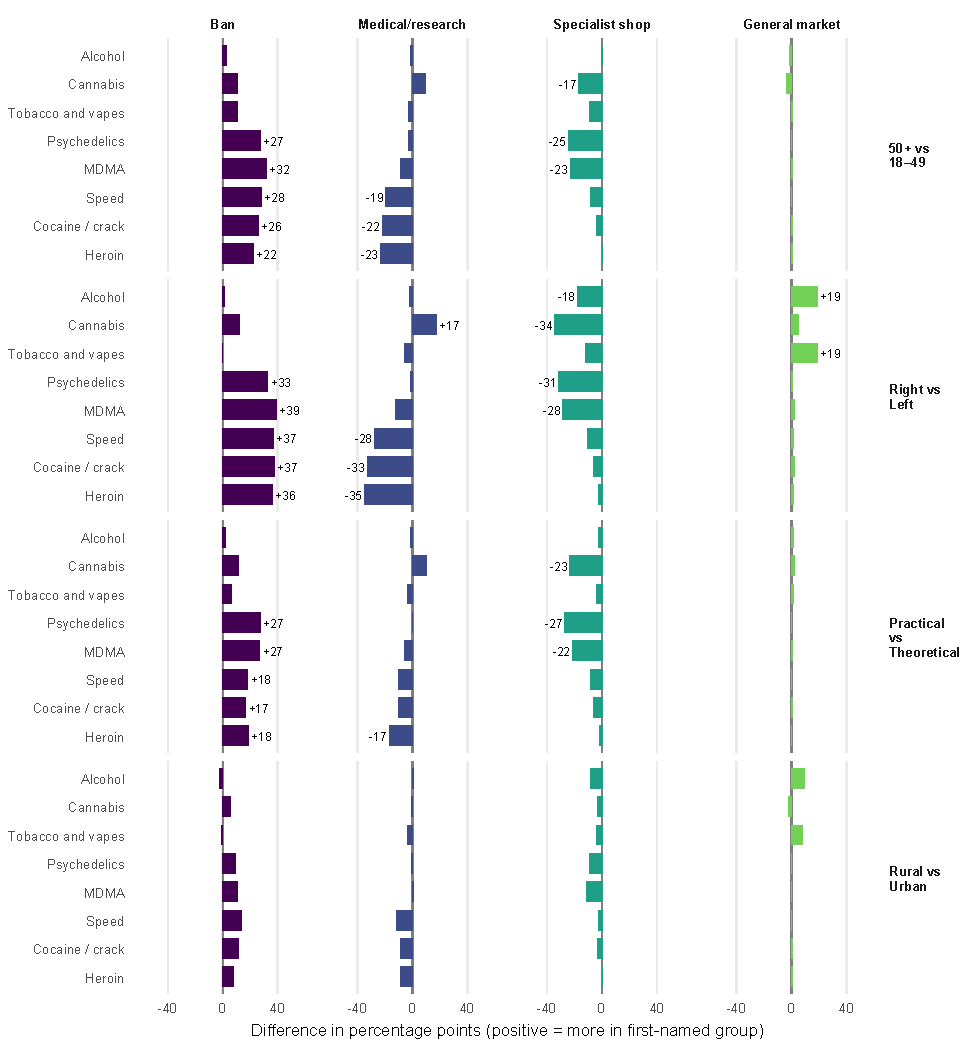
\includegraphics[width=\linewidth]{out/fig_regime_shifts.pdf}
  \caption{Older, right-wing, practically educated and rural respondents more often prefer a ban for every substance except alcohol and tobacco. Their counterparts instead favour a specialist shop for cannabis, psychedelics and MDMA, and medical or research supply for speed, cocaine and heroin. For alcohol and tobacco, right-wing and rural respondents favour a general market over a specialist shop. Each point is the difference in weighted share choosing a regime (percentage points) between two groups: age 50+ vs 18--49; vote right vs left; practical (incl.\ middle) vs theoretical education; rural (low or no urbanisation) vs urban (high or very high). Positive values: more among the older, right-wing, practically educated or rural group; per drug and demographic the four differences sum to zero. Grey bars span the four demographics; shaded cells mark where the pattern lies. Group sizes ($n$, unweighted): 50+ 714, 18–49 525; Right 394, Left 347; Practical 727, Theoretical 512; Rural 311, Urban 707. Vote: parties grouped into left, middle and right (provisional).}
  \label{fig:regime_shifts}
\end{figure}
